%* --- Options for printing (twoside) or digital (oneside) --- %
\newif\ifPRINTING
\PRINTINGtrue %! Set the conditional to true
%\PRINTINGfalse %! Set the conditional to false (one must be commented out)

\ifPRINTING
    \documentclass[british, twoside]{ntnuthesis}  % Language options: british, american, norsk, nynorsk
\else
    \documentclass[british, oneside]{ntnuthesis}  % Language options: british, american, norsk, nynorsk
\fi


%* --- Import of additional preamble files (advanced) --- %
\usepackage{import}  % import package allows for loading self-made .sty files
\usepackage{preamble/head_mk2}


%* --- Import support files --- %

%* Author
\author{Hauge, Max}
\shortauthor{MH}


%* Supervisor(s)
\newif\ifSINGLESUPERVISOR
%\SINGLESUPERVISORtrue  %! Set the conditional to true
\SINGLESUPERVISORfalse  %! Set the conditional to false

\ifSINGLESUPERVISOR
    \newcommand{\supervisorGrammar}{Supervisor}
    \newcommand{\supervisor_A}{Grepstad, Sigrid}
\else
    \newcommand{\supervisorGrammar}{Supervisors}
    \newcommand{\supervisorA}{Grepstad, Sigrid}
    \newcommand{\supervisorB}{Heap, Winston}  % For more supervisors add a new line here and update the titlepage_max.tex file
\fi


%* Title
\title{Tiling and Spectral Pairs for the \emph{d}-dimensional\\ Unit Cube}  %* sans serif
%\title{Tiling Sets and Spectral Pairs for the d-dimensional Unit Cube}  %* RM
%\title{Plaser Din Fancy Lange Tittel Her}  %* Original Placeholder
\shorttitle{Master's thesis}


%* Course name / Emnekode
\newcommand{\emnekode}{MA3911 — masteroppgave i matematiske fag}


%* Institutt
%? The command is the same no matter the language: bokmål, nynorsk, british, american
%? If changing between languages many times either update the "ntnuthesis.cls" file directly and comment out the code here
%? Or simply comment in/out the used/unused commands manually here each time you change the language
\renewcommand{\NTNUinstitutt}{Institute of Mathematical Sciences}
\renewcommand{\NTNUinstituttLowerC}{institute of mathematical sciences}


%* Date
\date{\today}
  %! Remember to update the content here
%
% From https://www.overleaf.com/learn/latex/Glossaries

\makeglossaries % Prepare for adding glossary entries


\newglossaryentry{latex}
{
        name=latex,
        description={Is a markup language especially suited for
scientific documents}
}

\newglossaryentry{bibliography}
{
        name=bibliography,
        plural=bibliographies,
        description={A list of the books referred to in a scholarly work,
typically printed as an appendix}
}

\newglossaryentry{maths}
{
    name=mathematics,
    description={Mathematics is what mathematicians do}
}


% --------------------
% ----- Acronyms -----
% --------------------

\newacronym{phd}{PhD}{philosophiae doctor}
\newacronym{CoPCSE}{CoPCSE@NTNU}{Community of Practice in Computer ScienceEducation at NTNU}
\newacronym{gcd}{GCD}{Greatest Common Divisor}
  % add glossary and acronym lists before document. Add \printglossaries after \tableofcontents to print

% * Commands for the document
% * -------------------------------------------------------------------
% * User-defined macros (functions) can go here, 
% * these may be overriden for each subfile by using \renewcommand{cmd}[args][default]{def} or simply \renewcommand{cmd}{def}



% * --- Layout & Graphics --- * %
%% Defines a new command for the horizontal lines. Change thickness here
\newcommand{\HRule}{\rule{\linewidth}{0.5mm}} 


%\renewcommand{\arraystretch}{1.25}  % For stretching tables and arrays


% * --- Crossreferencing --- * %
%% Avoids some words when crossreferencing to an enumerated list of equations within a theorem environment
%% Using \cref{thrm:my_theorem} \cref{eq:mt_c} will print "Theorem 2.0.2 (c)" and not "Theorem 2.0.2 Item (c)"
%% Original settings for both \crefname{} and \Crefname collected from cleverref pacakge .sty file
%\Crefname{enumi}{Item}{Items}%
%\Crefname{enumii}{Item}{Items}%
%\Crefname{enumiii}{Item}{Items}%
%\Crefname{enumiv}{Item}{Items}%
%\Crefname{enumv}{Item}{Items}%

\Crefname{enumi}{}{}%
\Crefname{enumii}{}{}%
\Crefname{enumiii}{}{}%
\Crefname{enumiv}{}{}%
\Crefname{enumv}{}{}%

\crefname{enumi}{}{}%
\crefname{enumii}{}{}%
\crefname{enumiii}{}{}%
\crefname{enumiv}{}{}%
\crefname{enumv}{}{}%


% * --- Mathematical symbol commands --- * %
% Arabic letters
\newcommand{\N}{\mathbb{N}}  % Already defined
\newcommand{\Z}{\mathbb{Z}}
\newcommand{\bbP}{\mathbb{P}}  % as \P yields some note P
\newcommand{\PP}{\mathbb{PP}}
\newcommand{\Q}{\mathbb{Q}}
\newcommand{\R}{\mathbb{R}}
\newcommand{\C}{\mathbb{C}}  % Already defined

\newcommand{\Fp}{\mathbb{F}_p}
\newcommand{\Fq}{\mathbb{F}_q}
\newcommand{\indic}{\mathbb{1}}

% Greek letters
\newcommand{\Tau}{\mathrm{T}}


% Z med striketrhough
\newcommand{\Zstroke}{\text{\ooalign{\hidewidth\raisebox{0.2ex}{--}\hidewidth\cr$Z$\cr}}}
\newcommand{\zstroke}{\text{\ooalign{\hidewidth -\kern-.3em-\hidewidth\cr$z$\cr}}}


% Degrees and-such
\newcommand{\degc}{$^\circ$C~}
\renewcommand{\deg}{\ensuremath{^{\circ}}}
\newcommand{\edegc}{^\circ \text{C}~}
\newcommand{\minone}{$^{-1}$}
\newcommand{\eminone}{^{-1}}


% Brackets
%% normal-brackets
\newcommand{\brac}[1]{(#1)}
\newcommand{\bracMed}[1]{\left(#1\right)}  % Husk at \left og \right legger på mellomrom. Ex: E (A) vs. E(A) 
%% Square-brackets
\newcommand{\bras}[1]{[#1]}
\newcommand{\brasMed}[1]{\left[#1\right]}
%% Curly-brackets
\newcommand{\braq}[1]{\{#1\}}
\newcommand{\braqMed}[1]{\left\{#1\right\}}
%% Angled-brackets
\newcommand{\braa}[1]{\langle#1\rangle}
\newcommand{\braaMed}[1]{\left \langle #1 \right \rangle}
%% Absolute values
\newcommand{\bral}[1]{|#1|}
\newcommand{\bralMed}[1]{\left|#1\right|}


% Operator names  
% A more high-level approach is to use \DeclareMathOperator{\max}{max} to create a shortcut with brackets and operator name at once, \max -> max(.)
\newcommand{\spn}[1]{\operatorname{span}\brac{#1}}
\newcommand{\spnMed}[1]{\operatorname{span}\bracMed{#1}}
\newcommand{\spnclos}[1]{\overline{\operatorname{span}}\brac{#1}}
\newcommand{\spnclosMed}[1]{\overline{\operatorname{span}}\bracMed{#1}}
\newcommand{\mes}[1]{\operatorname{mes}\brac{#1}}
\newcommand{\mesMed}[1]{\operatorname{mes}\bracMed{#1}}


\newcommand{\Cper}{C_{\text{per}}}

% others 
\newcommand{\inpl}[1]{\langle \lambda, #1 \rangle}
\newcommand{\indicator}[2]{\mathbb{1}_{#1}(#2)}
\newcommand{\indicatorNoVar}[1]{\mathbb{1}_{#1}}

% Set of exponential functions
\newcommand{\onedexp}{ \braq{e^{2\pi i \lambda t } : \lambda \in \Z} }
\newcommand{\alldexp}{ \braq{e^{2\pi i \inpl{t}} : \lambda \in \Z^d} }

% text replacements
\newcommand{\Ltwonorm}{$\|\cdot\|_{L^2}$-norm}  %! Uten dollartegn, rett i teksten
\newcommand{\LPnorm}{$\|\cdot\|_{L^p}$-norm}
\newcommand{\GenNormX}{$\|\cdot\|_{X}$-norm}
\newcommand{\GenNormH}{$\|\cdot\|_{H}$-norm}

% * --- Other Settings --- * %
% \newcommand{\masl}{m.a.s.l}

\newcommand{\defqed}{$\diamondsuit$}
\newcommand{\nsubset}{\not\subset}


\newcommand{\mycomment}[1]{}
  % add commands before document
\addbibresource{support_files/Mastergrad.bib}  % add the Bibliography file

%! Two-side option
%! Must manually check whether the page offset appears correctly on each 'left' and 'right' page. 
%? If the code is commented out (i.e. the offset appears on the wrong pages), then one also needs to update the headers in 'ntnuthesis.cls'
\ifPRINTING
    % The following code "flips" the offset for the 'left' and 'right' pages
    \let\tmp\oddsidemargin
    \let\oddsidemargin\evensidemargin
    \let\evensidemargin\tmp
    \reversemarginpar
\fi

%* —————————————  THE DOCUMENT  ————————————— %
\begin{document}
    %* --- Opening --- %
    %? Remember to comment out the title page when creating the final front page required by NTNU
    %% Title for the document
% --------------------------------------------------------------------------

\begin{titlepage}
	% Title
	\title{\textsf{Tiling and Spectral Pairs for the \emph{d}-dimensional\\ Unit Cube}}  %* sans serif
	%\title{Tiling Sets and Spectral Pairs for the d-dimensional Unit Cube}  %* RM
	%\title{Plaser Din Fancy Lange Tittel Her}  %* Original Placeholder
	\shorttitle{Masteroppgave}
	% Author
	\author{Hauge, Max}
	\shortauthor{MH}
	% Date
	\date{\today}

	\makeatletter
	\let\thetitle\@title
	\let\theauthor\@author
	\let\thedate\@date
	\makeatother


	\centering
    \vspace*{0.5 cm}
    % University Logo
    
\includegraphics[width=0.7\textwidth]{ntnu.png}\\[1.0 cm]
    
	% University Name
	\textsc{\LARGE \textsf{norwegian university of science and technology}}\\[1.0 cm]  %* sans serif no caps
    %\textsc{\LARGE Norwegian University of Science and Technology}\\[1.0 cm]  %* RM
    %\text{\LARGE norwegian university of science and technology}\\[1.0 cm]  %* RM Original Placeholder
    
	% Institute
	\textsc{\Large \textsf{institute of mathematical sciences}}\\[0.5 cm]  %* sans serif no caps
    %\textsc{\Large Institute of Mathematical Sciences}\\[0.5 cm]  %* RM
    %\text{\Large institute of mathematical sciences}\\[0.5 cm]  %* RM Original Placeholder
	
	% Course Name
	\textsc{\large \textsf{MA3911 — masteroppgave i matematiske fag}}\\[0.5 cm]  %* sans serif no caps
	%\textsc{\large MA3911 Masteroppgave i Matematiske Fag}\\[0.5 cm]  %* RM
    %\text{\large XXX 4242 MinEmnekode}\\[0.5 cm]  %* RM Original Placeholder
	
	%------------
	\rule{\linewidth}{0.2 mm} \\[0.4 cm]
	{ \LARGE \textbf{\uppercase{\thetitle}}}\\
	\rule{\linewidth}{0.2 mm} \\[1.0 cm]%[1.5 cm]
	
	

%! When the figure is used in the title, the figure environment is removed

%\begin{figure*}[h!]
%    \centering
    %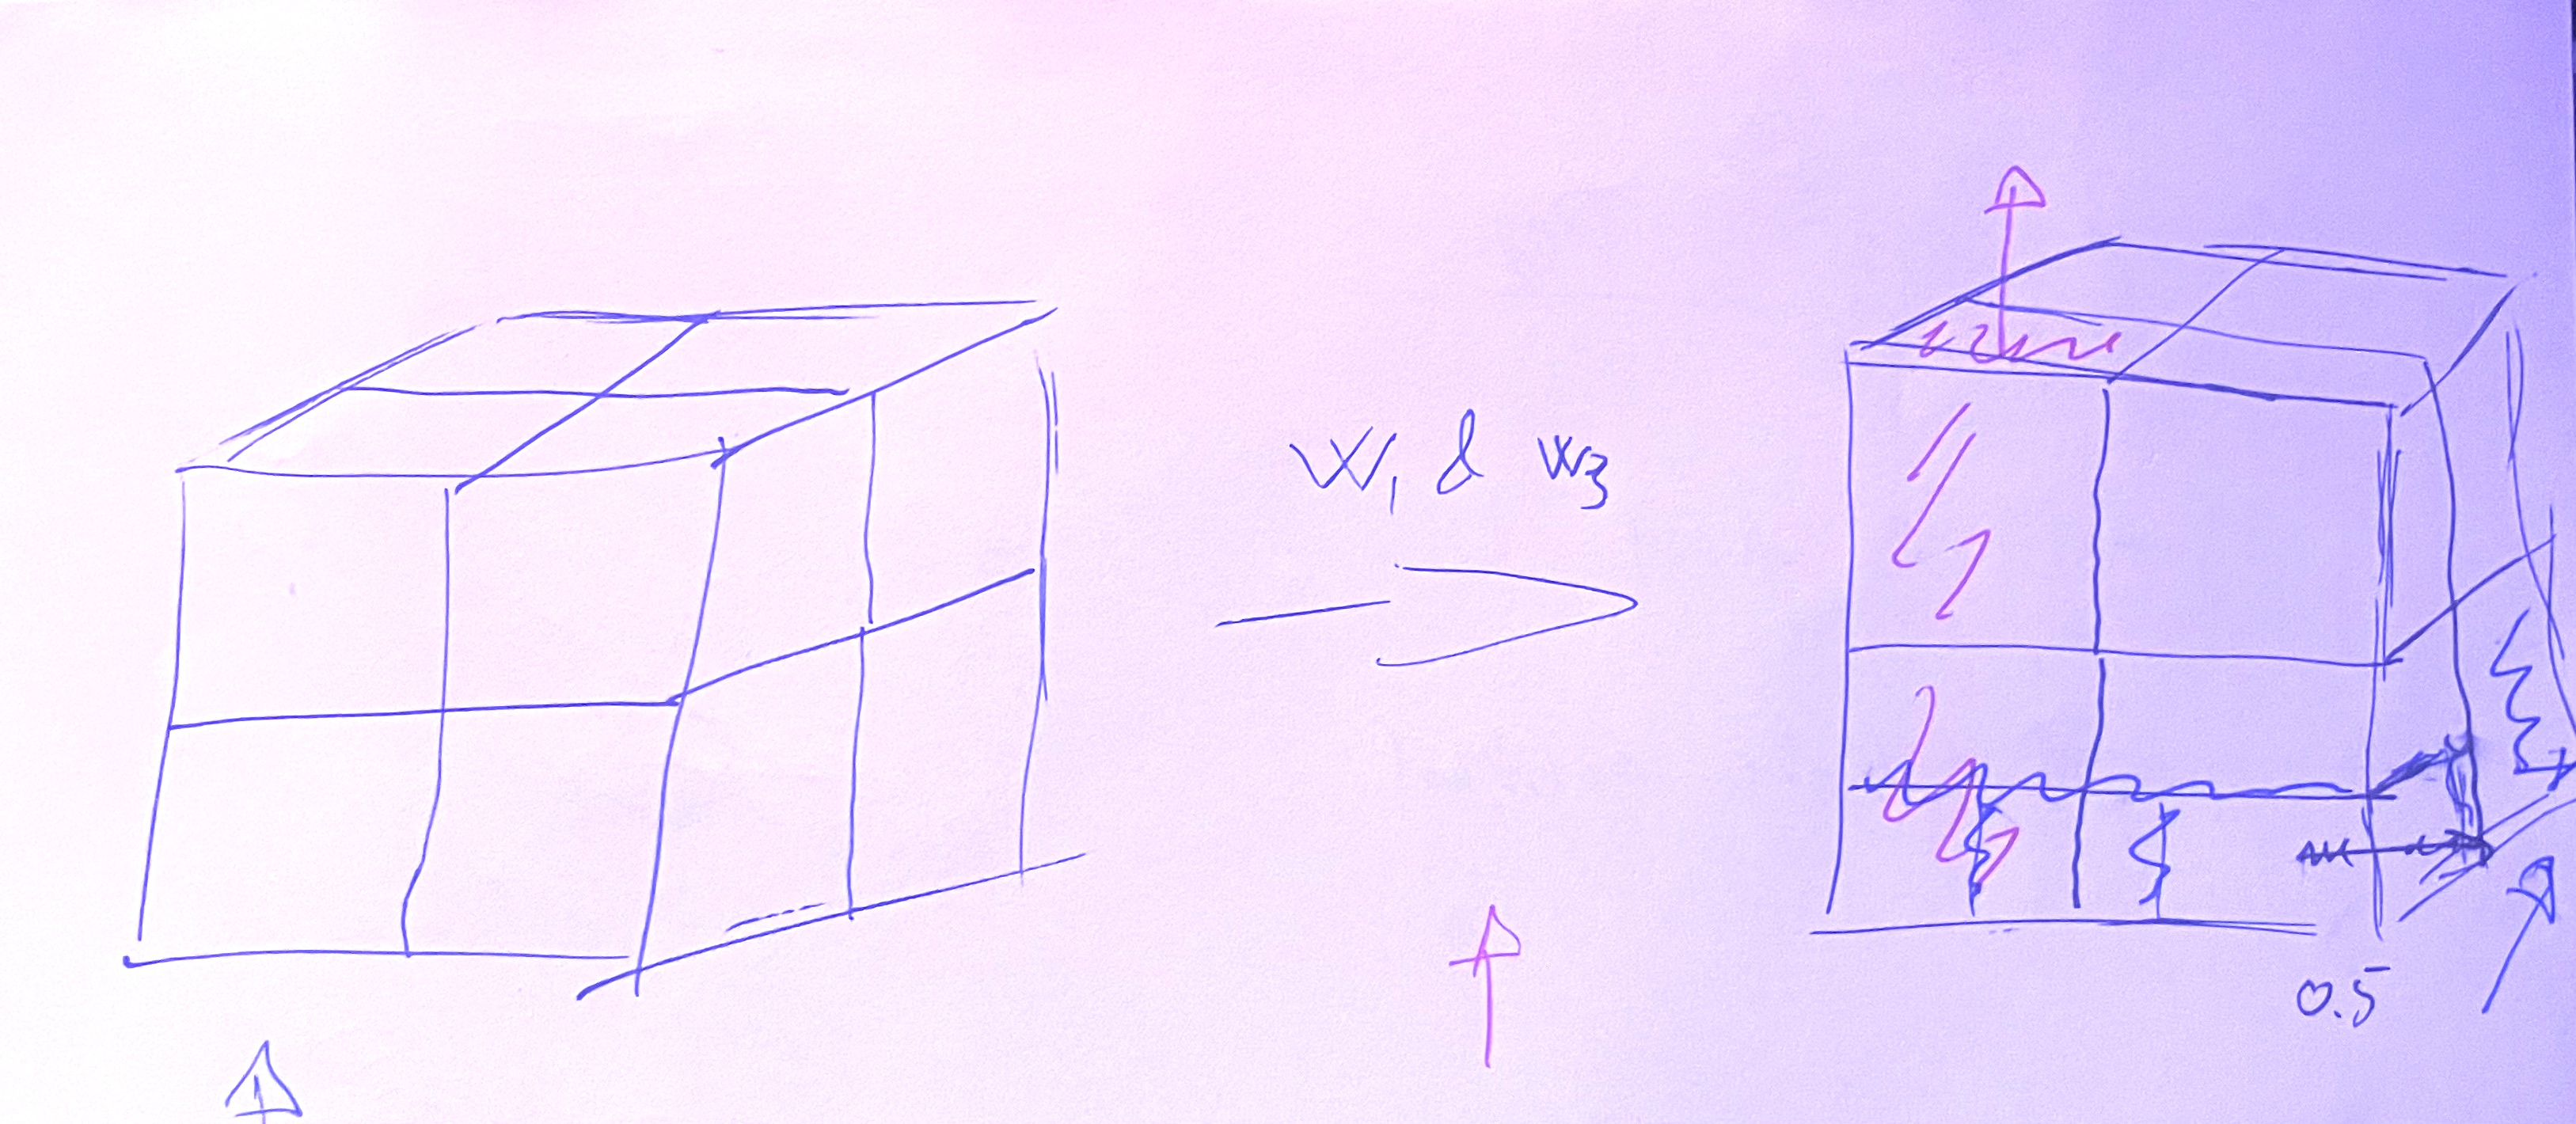
\includegraphics[width=0.87\linewidth]{aper_yeye.jpg}
    %* Figure
    % for the use in the online editor: \usepackage{tikz} 
    \begin{tikzpicture}[scale=0.9] %! The original scale is 1
        % Define the tile
        \def\tile{
        % Draw the unit cube
            \draw[black!95] (1,0,0) -- (1,0,1) -- (1,1,1) -- (1,1,0) -- cycle; % left face
            \draw[black!95] (0,0,0) -- (1,0,0) -- (1,0,1) -- (0,0,1) -- cycle; % bottom face
            \draw[black!95] (0,0,0) -- (0,1,0) -- (1,1,0) -- (1,0,0) -- cycle; % back face
            \draw[black!95, fill=gray!65] (1,0,0) -- (1,1,0) -- (1,1,1) -- (1,0,1) -- cycle; % right face
            \draw[black!95, fill=white] (0,0,1) -- (1,0,1) -- (1,1,1) -- (0,1,1) -- cycle; % front face
            \draw[black!95, fill=white](0,1,0) -- (0,1,1) -- (1,1,1) -- (1,1,0) -- cycle; % top face
        }

        \def\tilecolumn{
            % Draw the unit cube
                \draw[black!95] (1,0,0) -- (1,0,1) -- (1,1,1) -- (1,1,0) -- cycle; % left face
                \draw[black!95] (0,0,0) -- (1,0,0) -- (1,0,1) -- (0,0,1) -- cycle; % bottom face
                \draw[black!95] (0,0,0) -- (0,1,0) -- (1,1,0) -- (1,0,0) -- cycle; % back face
                \draw[black!95, fill=cyan] (1,0,0) -- (1,1,0) -- (1,1,1) -- (1,0,1) -- cycle; % right face
                \draw[black!95, fill=cyan] (0,0,1) -- (1,0,1) -- (1,1,1) -- (0,1,1) -- cycle; % front face
                \draw[black!95, fill=cyan](0,1,0) -- (0,1,1) -- (1,1,1) -- (1,1,0) -- cycle; % top face
            }
        
        \def\tilerow{
            % Draw the unit cube
                \draw[black!95] (1,0,0) -- (1,0,1) -- (1,1,1) -- (1,1,0) -- cycle; % left face
                \draw[black!95] (0,0,0) -- (1,0,0) -- (1,0,1) -- (0,0,1) -- cycle; % bottom face
                \draw[black!95] (0,0,0) -- (0,1,0) -- (1,1,0) -- (1,0,0) -- cycle; % back face
                \draw[black!95, fill=orange] (1,0,0) -- (1,1,0) -- (1,1,1) -- (1,0,1) -- cycle; % right face
                \draw[black!95, fill=orange] (0,0,1) -- (1,0,1) -- (1,1,1) -- (0,1,1) -- cycle; % front face
                \draw[black!95, fill=orange](0,1,0) -- (0,1,1) -- (1,1,1) -- (1,1,0) -- cycle; % top face
            }
    
        % Draw the tiling pattern LEFT: x = 0,1,2,3
        % not shifted
        % the backseat boys
        \foreach \x in {0,1,2,3}{
            \foreach \y in {-2,-1,0,1}{
                \foreach \z in {-2,-1}{
                    \pgfmathsetmacro{\shiftX}{\x}
                    \pgfmathsetmacro{\shiftY}{\y}
                    \pgfmathsetmacro{\shiftZ}{\z}
                    
                    \begin{scope}[shift={(\shiftX,\shiftY,\shiftZ)}]
                    \tile % Draw the tile
                    \end{scope}
                }
            }
        }
        % Draw the back four cubes as two rows for the shift in X
        % not shifted
        \foreach \x in {0,1,2,3}{
            \foreach \y in {-2,-1,0}{
                \foreach \z in {0}{
                    \pgfmathsetmacro{\shiftX}{\x}
                    \pgfmathsetmacro{\shiftY}{\y}
                    \pgfmathsetmacro{\shiftZ}{\z}
                    
                    \begin{scope}[shift={(\shiftX,\shiftY,\shiftZ)}]
                    \tile % Draw the tile
                    \end{scope}
                }
            }
        }
        % Will be shifted – in the X direction
        \foreach \x in {0,1,2,3}{
            \foreach \y in {1}{
                \foreach \z in {0}{
                    \pgfmathsetmacro{\shiftX}{\x}
                    \pgfmathsetmacro{\shiftY}{\y}
                    \pgfmathsetmacro{\shiftZ}{\z}
                    
                    \begin{scope}[shift={(\shiftX,\shiftY,\shiftZ)}]
                    \tilerow % Draw the tile
                    \end{scope}
                }
            }
        }
        
        
        % not shifted
        \foreach \x in {0}{
            \foreach \y in {-2,-1,0,1}{
                \foreach \z in {1}{
                    \pgfmathsetmacro{\shiftX}{\x}
                    \pgfmathsetmacro{\shiftY}{\y}
                    \pgfmathsetmacro{\shiftZ}{\z}
                    
                    \begin{scope}[shift={(\shiftX,\shiftY,\shiftZ)}]
                    \tile % Draw the tile
                    \end{scope}
                }
            }
        }
        % Draw the front four cubes as two columns for the shift in Y
        % Will be shifted – in the Y direction
        \foreach \x in {1}{
            \foreach \y in {-2,-1,0,1}{
                \foreach \z in {1}{
                    \pgfmathsetmacro{\shiftX}{\x}
                    \pgfmathsetmacro{\shiftY}{\y}
                    \pgfmathsetmacro{\shiftZ}{\z}
                    
                    \begin{scope}[shift={(\shiftX,\shiftY,\shiftZ)}]
                    \tilecolumn % Draw the tile
                    \end{scope}
                }
            }
        }
        % not shifted
        \foreach \x in {2,3}{
            \foreach \y in {-2,-1,0,1}{
                \foreach \z in {1}{
                    \pgfmathsetmacro{\shiftX}{\x}
                    \pgfmathsetmacro{\shiftY}{\y}
                    \pgfmathsetmacro{\shiftZ}{\z}
                    
                    \begin{scope}[shift={(\shiftX,\shiftY,\shiftZ)}]
                    \tile % Draw the tile
                    \end{scope}
                }
            }
        }
        
        % Draw the Inbetween stuff
        %———————————————————————————————————
        \draw[->, thick, black] (5.5,0.2) -- (7.5,0.2);
        \node[black] at (6.6,0.5) {\Large $\upsilon',\upsilon''$}; 
        
        
        
        
        % Draw the tiling pattern RIGHT: x= 9,10,11,12
        %———————————————————————————————————
        % not shifted
        % the backseat boys
        \foreach \x in {9,10,11,12}{
            \foreach \y in {-2,-1,0,1}{
                \foreach \z in {-2,-1}{
                    \pgfmathsetmacro{\shiftX}{\x}
                    \pgfmathsetmacro{\shiftY}{\y}
                    \pgfmathsetmacro{\shiftZ}{\z}
                    
                    \begin{scope}[shift={(\shiftX,\shiftY,\shiftZ)}]
                    \tile % Draw the tile
                    \end{scope}
                }
            }
        }
        % Draw the back four cubes as two rows for the shift in X
        % not shifted
        \foreach \x in {9,10,11,12}{
            \foreach \y in {-2,-1,0}{
                \foreach \z in {0}{
                    \pgfmathsetmacro{\shiftX}{\x}
                    \pgfmathsetmacro{\shiftY}{\y}
                    \pgfmathsetmacro{\shiftZ}{\z}
                    
                    \begin{scope}[shift={(\shiftX,\shiftY,\shiftZ)}]
                    \tile % Draw the tile
                    \end{scope}
                }
            }
        }
        % Will be shifted – in the X direction
        \foreach \x in {8,9,10,11,12}{
            \foreach \y in {1}{
                \foreach \z in {0}{
                    \pgfmathsetmacro{\shiftX}{\x+0.5}
                    \pgfmathsetmacro{\shiftY}{\y}
                    \pgfmathsetmacro{\shiftZ}{\z}
                    
                    \begin{scope}[shift={(\shiftX,\shiftY,\shiftZ)}]
                    \tilerow % Draw the tile
                    \end{scope}
                    
                    %\ifnum\x=9
                    %    \draw[->, orange] (\shiftX+1,1.4) --node[below] {$0.5$} (\shiftX+2,1.4);             \fi
                }
            }
        }
        

        % not shifted
        \foreach \x in {9}{
            \foreach \y in {-2,-1,0,1}{
                \foreach \z in {1}{
                    \pgfmathsetmacro{\shiftX}{\x}
                    \pgfmathsetmacro{\shiftY}{\y}
                    \pgfmathsetmacro{\shiftZ}{\z}
                    
                    \begin{scope}[shift={(\shiftX,\shiftY,\shiftZ)}]
                    \tile % Draw the tile
                    \end{scope}
                }
            }
        }
        % Draw the front four cubes as two columns for the shift in Y
        % Will be shifted – in the Y direction
        \foreach \x in {10}{
            \foreach \y in {-3,-2,-1,0,1}{
                \foreach \z in {1}{
                    \pgfmathsetmacro{\shiftX}{\x}
                    \pgfmathsetmacro{\shiftY}{\y+0.5}
                    \pgfmathsetmacro{\shiftZ}{\z}
                    
                    \begin{scope}[shift={(\shiftX,\shiftY,\shiftZ)}]
                    \tilecolumn % Draw the tile
                    \end{scope}
                    
                    %\ifnum\y=1
                    %    \draw[->, thick, cyan] (7,\shiftY+0.5) --node[right] {$0.5$} (7,\shiftY+1.5);             \fi
                }
            }
        }
        % not shifted
        \foreach \x in {11,12}{
            \foreach \y in {-2,-1,0,1}{
                \foreach \z in {1}{
                    \pgfmathsetmacro{\shiftX}{\x}
                    \pgfmathsetmacro{\shiftY}{\y}
                    \pgfmathsetmacro{\shiftZ}{\z}
                    
                    \begin{scope}[shift={(\shiftX,\shiftY,\shiftZ)}]
                    \tile % Draw the tile
                    \end{scope}
                }
            }
        }
        
        
  
    \end{tikzpicture}
    %\caption{Illisustrated in the \cref{fig:big_aperi} is simply a bigger version of the aperiodic tile we have constructed.}
    %\label{fig:big_aperi}
%\end{figure*}


	% Page setup
	\begin{minipage}{0.4\textwidth}
		\begin{flushleft} \large
			\emph{Author:}\\
			\textrm{\theauthor}
		\end{flushleft}
	\end{minipage}
	\begin{minipage}{0.4\textwidth}
		\begin{flushright} \large
			\emph{Supervisor:} \\
			\textrm{Grepstad, Sigrid}\\  % Supervisor #1
			\textrm{Heap, Winston} %>\\  % Supervisor #2
		\end{flushright}
	\end{minipage}\\[1 cm]
	

	{\large \thedate}%\\[2 cm]
 
	%\vfill
	
\end{titlepage}  %! Temporary title page for your project
    
%? Note: We have "Clearpage" automatically after the title page

%* Abstract
\thispagestyle{plain}


\addcontentsline{toc}{chapter}{Abstract}
\clearpage


%* Preface & acknowledgements
\ifPRINTING
    % This puts the quote on the "left double page with the Preface on the right"
    
% Adjust margins if needed
\ifPRINTING
    \newgeometry{top=0.5in, bottom=0.5in, left=1in, right=1in, bindingoffset=6mm}
\else
    \newgeometry{top=0.5in, bottom=0.5in, left=1in, right=1in}
\fi


\thispagestyle{empty} % Remove page number


\vspace*{\fill}
\begin{center}
    \textit{\enquote{Oh, he seems like an okay person, except for being a little strange in some ways. All day he sits at his desk and scribbles, scribbles, scribbles. Then, at the end of the day, he takes the sheets of paper he's scribbled on, scrunches them all up, and throws them in the trash can.}}\\
\end{center}
\begin{flushright}
    \textbf{— J. von Neumann's housekeeper, describing her employer}
\end{flushright}
\vspace*{\fill}

\restoregeometry % Restore original page margins

    \chapter*{Preface}
    


%\phantomsection
%\addcontentsline{toc}{chapter}{Preface}


%\begin{center}
\vspace{.25in}


TEXt TEXt

acknowledgments 

%* Overview thing with little details. Instead of rewriting everything. You have a nice informal discussion within the chapters. 
%* Mention Mikowsky in the intro when I go through the contents. And mention that it will not be the focus here. 


%\end{center}
\else
    % This puts the quote on the page after the Preface
    \chapter*{Preface}
    


%\phantomsection
%\addcontentsline{toc}{chapter}{Preface}


%\begin{center}
\vspace{.25in}


TEXt TEXt

acknowledgments 

%* Overview thing with little details. Instead of rewriting everything. You have a nice informal discussion within the chapters. 
%* Mention Mikowsky in the intro when I go through the contents. And mention that it will not be the focus here. 


%\end{center}
    
% Adjust margins if needed
\ifPRINTING
    \newgeometry{top=0.5in, bottom=0.5in, left=1in, right=1in, bindingoffset=6mm}
\else
    \newgeometry{top=0.5in, bottom=0.5in, left=1in, right=1in}
\fi


\thispagestyle{empty} % Remove page number


\vspace*{\fill}
\begin{center}
    \textit{\enquote{Oh, he seems like an okay person, except for being a little strange in some ways. All day he sits at his desk and scribbles, scribbles, scribbles. Then, at the end of the day, he takes the sheets of paper he's scribbled on, scrunches them all up, and throws them in the trash can.}}\\
\end{center}
\begin{flushright}
    \textbf{— J. von Neumann's housekeeper, describing her employer}
\end{flushright}
\vspace*{\fill}

\restoregeometry % Restore original page margins

\fi


%* Table of contents
\setcounter{tocdepth}{3}
\tableofcontents

% Blank page to avoid having Chapter 1 and TOC on the same "double page"
\ifPRINTING
    \newpage
    \thispagestyle{empty}
    \vspace*{\fill}
    \clearpage
\fi



    %* --- DOCUMENT START --- %
    %? --- NOTE: Folder structure --- %
    % 1. Allows compilation of each subfile rather than compiling everything at once each time
    % 2. Subfiles must have this file as an option while using the "documentclass" subfile
    % 3. Loading a subfile is done with \subfile{"path-to-file"}
    % 4. Remember to use the template to get all the right \subfile commands in each .tex document
    % ---
    
    % Chapter 1
    \chapter{Introduction}
        \subfile{chapters/01_introduction.tex}
    
    % Chapter 2
    \chapter{Notation and Preliminaries}
        \subfile{chapters/02_preliminaries.tex}
    
    % Chapter 3
    \chapter{Tiles and tiling sets}\label{chap:tiling}
        \subfile{chapters/03_tilings.tex}

    % Chapter 4
    \chapter{Spectral sets and spectra}
        \subfile{chapters/04_spectral_sets.tex}
    
    % Chapter 5
    \chapter{Equivalence of spectra and tiling sets}\label{chap:equivalence}
        \subfile{chapters/06_equiv_tiling_spec_ncube.tex}

    % Bibliography
    \printbibliography

    %! Two-side option
    %! Must manually check whether the last page of the bibliography ends on the "left" or "right" side of the "double page".
    %! The back cover from NTNU should be "alone" when using the "two-page" view mode in the PDF reader. 
    \ifPRINTING
    \newpage
    \thispagestyle{empty}
    \vspace*{\fill}
    \clearpage
    \fi
\end{document}
